\documentclass{jarticle}
% \usepackage{flushend}  % 最終ページの2カラムの左右の高さを揃える
\usepackage[dvipdfmx]{graphicx}
\usepackage{subcaption}
\captionsetup[figure]{justification=centering}
\captionsetup[table]{justification=centering}
\usepackage[ipa]{pxchfon}
\usepackage{otf}
\renewcommand{\figurename}{図~}
\renewcommand{\tablename}{表~}
\newcommand{\figref}[1]{\figurename\ref{#1}}
\newcommand{\tabref}[1]{\tablename\ref{#1}}
\usepackage{robomech}
% \usepackage[dvipdfmx,setpagesize=false]{hyperref}



\begin{document}
\makeatletter
\title{視覚と行動のend-to-end学習により\\経路追従行動をオンラインで模倣する手法の提案}
{― データセット収集密度の動的調整による学習の効率化 ―}
{A Proposal for an Online Imitation Method of
Path-tracking\\ Behavior by End-to-end Learning of Vision and Action}
{- Efficiency Improvement of Learning by Dynamic Adjustment of Dataset Collection Density -}

\author{
\begin{tabular}{c}
 \hspace*{0.3zw}○学\hspace{1zw}今井悠月 (千葉工大)\hspace{2zw}正\hspace{1zw}上田隆一 (千葉工大)\hspace{2zw}正\hspace{1zw}林原靖男(千葉工大)\\
 \end{tabular}
 \vspace{1zh} \\
 \begin{tabular}{l}
 {\hspace*{4zw}\small Yuzuki IMAI, Chiba Institute of Technology, s20c1015as@s.chibakoudai.jp}\\
 {\hspace*{4zw}\small Ryuichi UEDA, Chiba Institute of Technology}\\
 {\hspace*{4zw}\small Yasuo HAYASHIBARA, Chiba Institute of Technology}\\
\end{tabular}
}
\makeatother

\abstract{ \small 
We have proposed a method for path-tracking of autonomous mobile robots by end-to-end learning of vision and action. Our method aims to diversify the navigation methods for these robots. It involves collecting a dataset while the robot moves and using this for learning. However, the density of data collection has not been discussed, and the density is uniform. This may result in excessive data collection in certain route areas. Addressing this, we first check for any bias in the collected dataset. We then propose a method to adjust the data collection density by varying the robot's translational speed based on the training data. The effectiveness of our proposed method is confirmed through experiments in a simulator.
}

\date{} % 日付を出力しない
\keywords{Autonomous mobile robot, End-to-end learning, Navigation, Dataset}

\maketitle
\thispagestyle{empty}
\pagestyle{empty}

\small
\section{緒言}
本研究グループは,移動ロボットを対象に,従来からカメラ画像とロボットの角速度を end-to-end 学習することで,経路追従する手法を
提案し,その有効性を検証してきた\cite{okada}\cite{okada2}\cite{kiyooka}.
これには,移動ロボットのナビゲーション手段を複数化するというねらいがある.
本手法は,地図に基づく経路追従行動を,画像を入力とする行動に模倣する.
地図に基づく経路追従とは,あらかじめ作成した地図と LiDAR,オドメトリなどを用いて,自己位置推定,
経路計画,制御などの複数のタスクを実行し,経路追従する方法である.
本手法を用いることで,ロボットは地図に基づく経路追従と同じ行動を,画像のみで行えるようになる.
よって,地図に基づく経路追従と画像に基づく経路追従の 2 つのナビゲーション手段を獲得できる.
これらを状況に応じて高い信頼性が見込まれる方を選択することで,経路追従を継続できる可能性が高まる.\\
\hspace*{1zw}本研究と同様に,カメラ画像を入力として,end-to-end 学習により経路追従する手法は,いくつか
提案されている.
例えば,Muller らは,人のコントローラ操作と画像を end-to-end 学習することで,オフロード環境で障害物を
回避して走行できることを確認した\cite{off_load}.また,Moridian らは,人のコントローラ操作と画像,測域
センサのデータを end-to-end 学習することで,一定の経路を走行できることを確認した\cite{Moridian}.
さらに,Bojarski らは,画像と人が操作したステアリングの角度を end-to-end 学習することで,自動運転する
手法を提案した\cite{Bojarski}.
これらの手法はすべて人の操作を教師データとしているのに対し,本手法はルールベースの制御器の出力である
角速度を教師データとしている.そのため,すでに制御器が1つ以上存在する必要があり,適用範囲は狭くなるが,
データセットの収集に人の操作が不要である.
それに加えて,ロボットが常に目標経路に復帰する行動を収集できるため,人の操作を教師データと
する場合よりも,経路追従を継続しやすいことが確認されている\cite{imai}.\\
\hspace*{1zw}ここで,本手法はロボットを走行させながら,データセットを収集し,
それを用いて学習するが,データセットを収集する密度に関してはこれまで議論されていない.
これまでの実験では,ロボットの並進速度は常に一定(0.2 m/s)としており,目標経路に対して,
常に同じ密度でデータセットを収集している.
しかし,一般的な環境で目標経路の多くを占める直線的な経路では,過剰にデータを収集しているおそれがある.
収集したデータセットは,各ステップごとに無作為に取り出され,それを学習に
用いるため,割合の多いデータは多く学習され,割合の少ないデータはあまり学習されていない.
つまり,データの割合が少ない部分でも経路追従行動を得るには,多くの訓練時間を要する.
よって,収集および学習されるデータの偏りを少なくし,学習を効率化することが望まれる.\\
\hspace*{1zw}これを踏まえ,本稿では,まず従来手法における実験結果の一例を取り上げ,
収集および学習されるデータセットに偏りがあるかを確認する.
そのうえで,データセットの収集密度を調整し,学習を効率化するために,
ロボットの並進速度を教師データの値に応じて可変にする手法を提案する.
なお,学習を効率化する手法は,これまでに本研究グループでもいくつか提案されている.
例えば,藤原らは,オーバーサンプリングによりデータの不均衡を改善する手法を提案した\cite{fuji}.
また,\CID{8705}橋らは,データを事前に収集し,オフラインで学習する手法を提案した\cite{takahashi}.
さらに,今井らは,モデルの評価に基づき訓練を打ち切る手法を提案した\cite{imai2}.
いずれの手法も訓練時間の短縮に成功しているが,ロボットの並進速度は常に一定としている.\\
\hspace*{1zw}本稿では,今井らの手法を採用し,シミュレータで実験する.
ロボットの並進速度を可変にする場合と,そうでない場合で結果を比較することにより,
提案手法の有効性を検証する.


\section{end-to-end 学習により経路追従行動を模倣する手法}
本研究グループが従来から提案する手法について述べる.
本手法は end-to-end 学習を用いて,地図に基づく経路追従行動を,視覚を入力とする行動にオンラインで模倣する.
はじめに地図に基づく経路追従を模倣学習する手法について述べた後,訓練済みモデルを用いた視覚に基づく
経路追従手法について述べる.

\subsection{地図に基づく経路追従の模倣学習}
地図に基づく経路追従を模倣学習するシステムを\figref{fig:3}に示す.
学習時には,ルールベースの制御器を用いて,ロボットは自律移動する.
それと同時に,64$×$48に リサイズした画像とルールベースの制御器から出力される
ヨー方向の目標角速度をペアにしたデータセットを収集し,end-to-end で学習する.
本研究グループでは,ルールベースの制御器に ROS navigation パッケージ\cite{navigation}を採用している.
ROS navigation パッケージは,並進速度と角速度を出力するが,角速度のみを教師データとしている.
データセットの収集と学習は一定時間(0.2 s)ごとに繰り返すが,これを 1ステップとしており,
1 ステップにつき,収集したデータセットの中から 8 個のデータを取り出して学習する.
学習には Experience Replay を採用する.ネットワークは\figref{fig:2}に示すように,
左から順に,入力層 1,畳み込み層 3,全結合層 2,出力層 1 の全 7 層で構成されたものを用いる.\\
\hspace*{1zw}また,他の研究\cite{Moridian}\cite{Bojarski}に倣い,
データセットの収集には 3つのカメラ(左・中央・右)を用いる.
この時,\tabref{table:1}のように,左右のカメラ画像に対応する目標角速度には,
それぞれ目標経路に戻るようにオフセットを加える.
具体的には,左のカメラには目標角速度に 0.2 rad/s を引いた値を,
右のカメラには目標角速度に 0.2 rad/s を足した値を教師データとする.
これにより,データの量を増やすことや,過学習を防ぐ効果が期待される.
ただし,旋回時(0.1 rad/s 以上)には,中央のカメラのみを使用する.\\
\hspace*{1zw}ロボットのモータを制御するモジュールは,ROS  navigation パッケージから出力される
角速度と,学習器から出力される角速度の 2つがあり,切り替えることが可能である.
岡田らの手法\cite{okada}に倣い,学習器の出力をベースに走行する.
このようにすることで,学習が不足している部分で,ロボットは目標経路から外れることになるため,
目標経路へ復帰する行動をより効率的に収集できる.

\begin{figure}[h!]
  \centering
   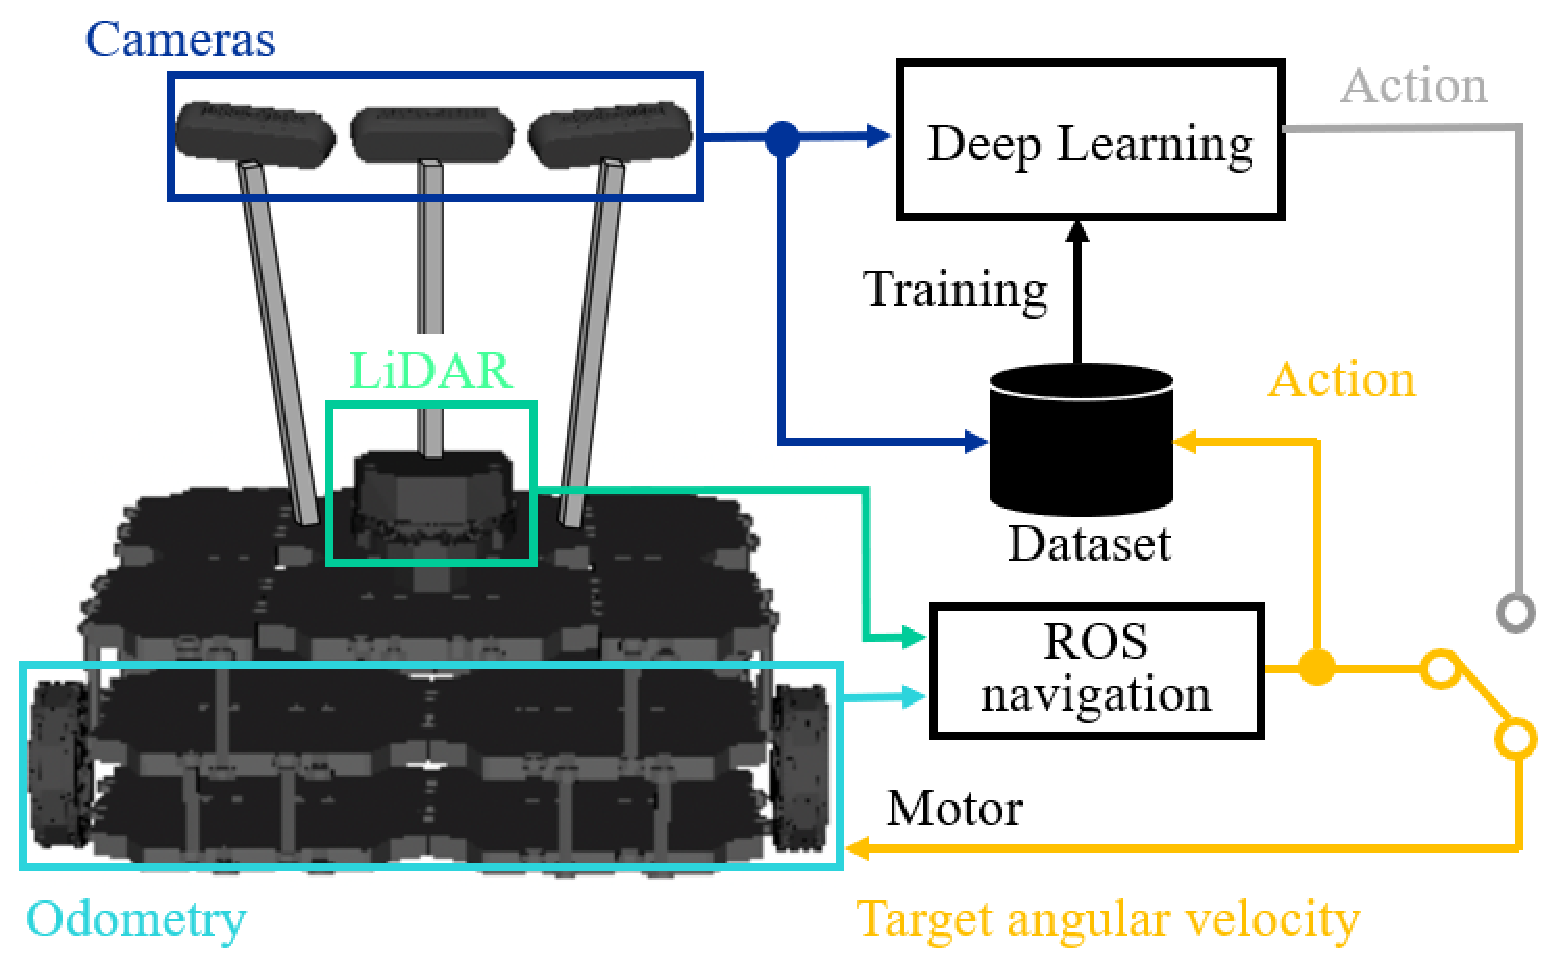
\includegraphics[height=54mm]{./pdf/learn.pdf}
   \caption{Method to imitate path-tracking behavior}
   \label{fig:3}
\end{figure}


\begin{figure}[h!]
  \centering
   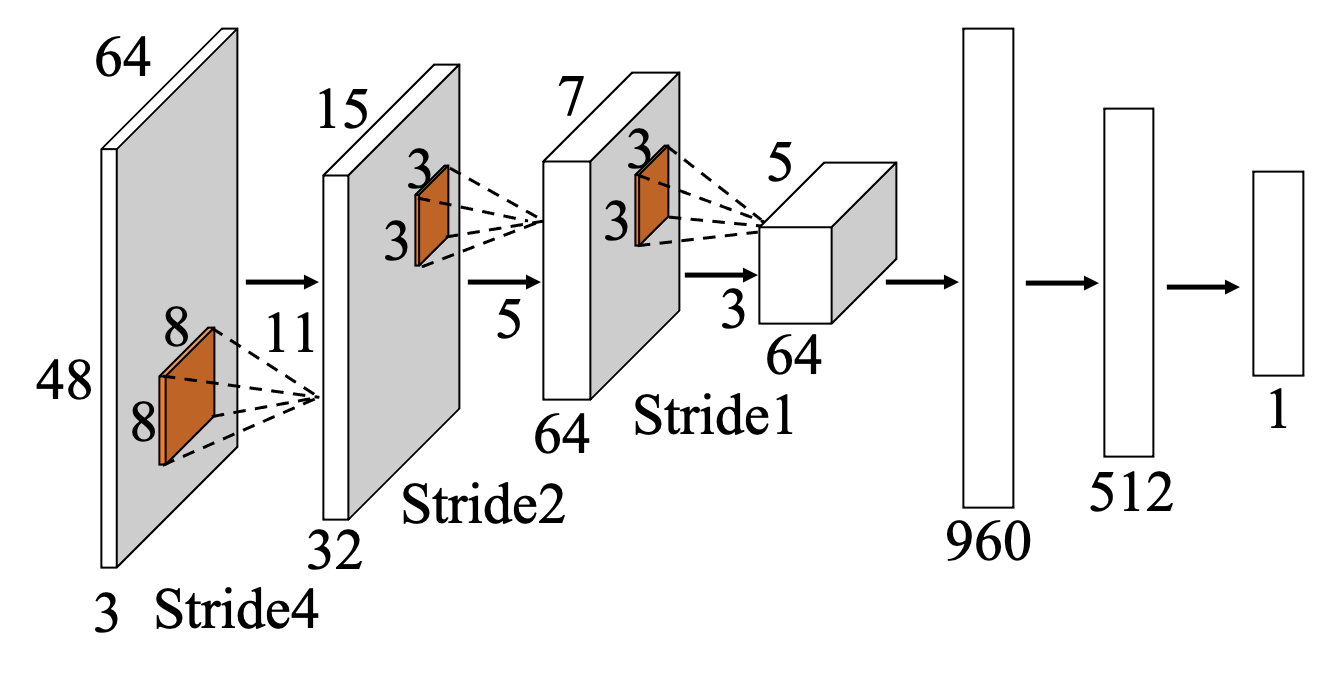
\includegraphics[height=44mm]{pdf/network.pdf}
   \caption{Structure of network}
   \label{fig:2}
\end{figure}

\begin{table}[h!]
  \centering
  \caption{Yaw angular velocity offset}
  \label{table:1}
    \scalebox{0.96}[0.96]{
    \begin{tabular}{|l||l|}
      \hline
      Cameras & Yaw angular velocity offset (rad/s)\\
      \hline\hline
      Left camera & ROS navigation system output $-$ 0.2\\
      \hline
      Center camera & ROS navigation system output\\
      \hline
      Right camera & ROS navigation system output $+$ 0.2\\
      \hline
    \end{tabular} }
\end{table}






\subsection{訓練済みモデルを用いた視覚に基づく経路追従}
学習が終了したら,訓練済みモデルを用いて,経路追従できるかを確認する.
このときのシステムを\figref{fig:4}に示す.
ここでは,ROS の navigation パッケージからの出力は使用せずにロボットを制御する.
画像を学習器に入力し,その推定結果をヨー方向の目標角速度としてロボットを自律移動させる.
ロボットのヨー方向の角速度には学習器の出力を用いるが,並進速度は常に一定 (0.2 m/s) とする.
また,地図に基づく経路追従の模倣学習時には, 3 つのカメラ(左・中央・右)を用いたが,
訓練済みモデルを用いた視覚に基づく経路追従時には, 3 つのカメラのうち,中央のカメラのみを使用する.

\begin{figure}[h!]
  \centering
   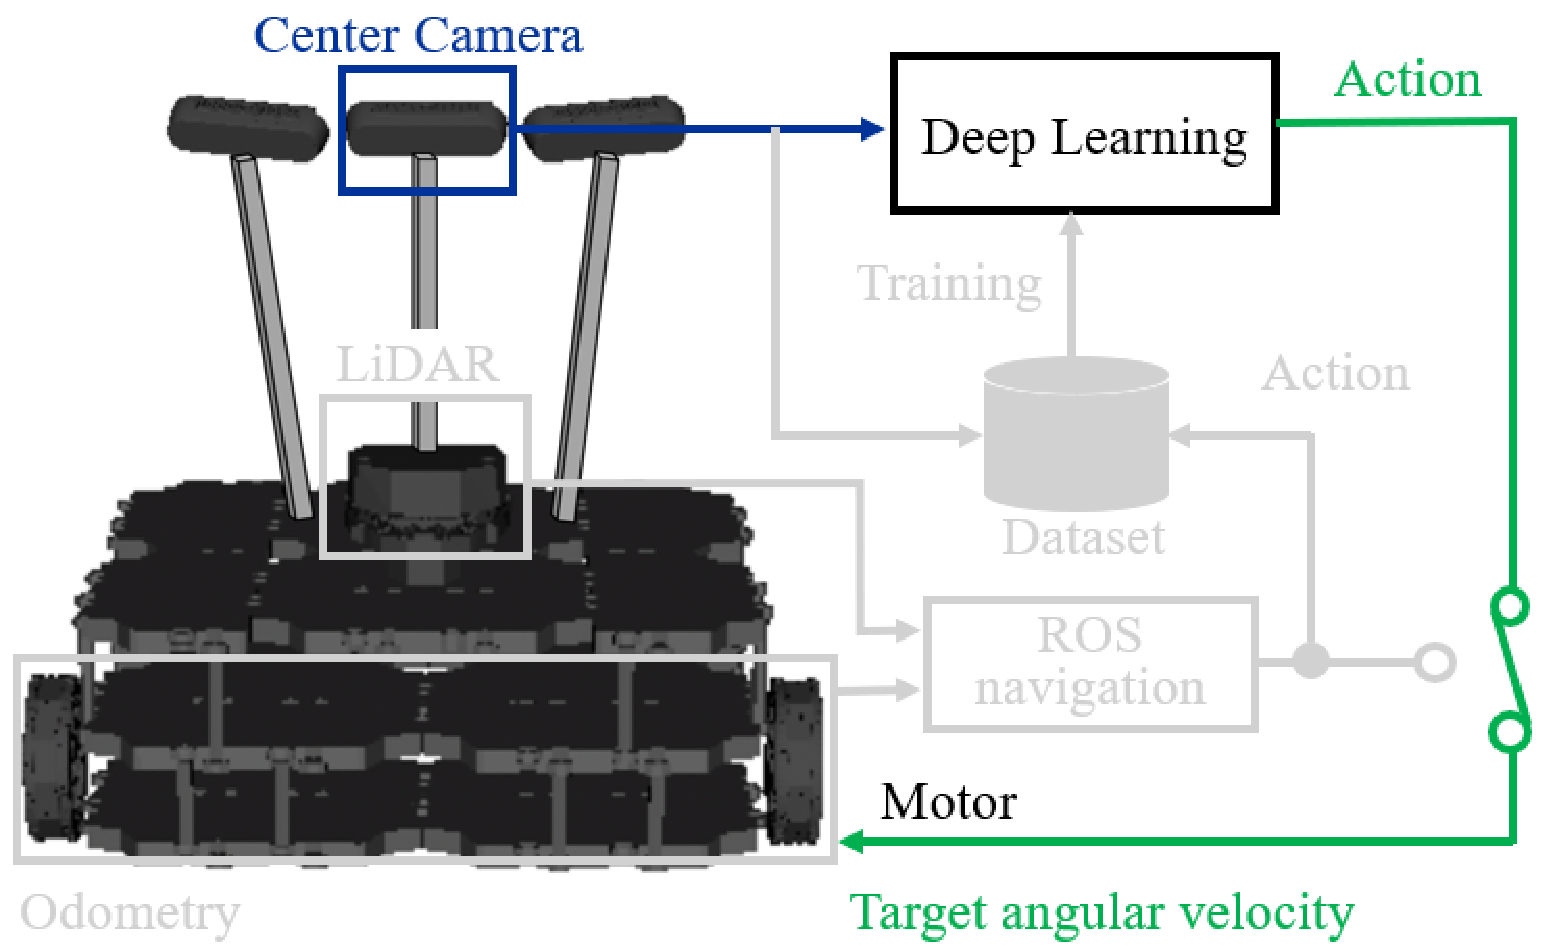
\includegraphics[height=53mm]{./pdf/afterlearn.pdf}
   \caption{Vision-based path-tracking using learned model}
   \label{fig:4}
\end{figure}

\section{モデルの評価に基づき訓練を打ち切る手法}
本稿の実験で採用する,今井らが提案した手法について述べる.\figref{fig:5}に本手法のシステムを示す.
2.1節で述べた地図に基づく経路追従の模倣学習手法に,訓練中のモデルを評価し,
望む出力がある程度得られたと判定したら,訓練を終了する仕組みを追加している.
具体的には,ROS navigation パッケージの出力である角速度と,学習器の出力である角速度を比較する.
比較の結果,その差の絶対値が一定値(0.05 rad/s)未満であれば,その地点において望ましい出力が得られている
と判定する.この点を DOL(desired output location)と呼び,判定をステップごとに繰り返す.
データセットを収集しつつ,学習し, DOL の割合が一定値を超えたところで訓練を打ち切る.
これにより,従来は一定のステップ数を用いていた訓練を,訓練の結果に応じて適切なステップ数で打ち切る.
ただし,経路の一部でも DOL が少ないと経路追従できないため,DOL の割合は経路全体に対して
ではなく,経路を分割して算出する.
以降,本手法を従来手法と呼ぶこととする.

\begin{figure}[h!]
  \centering
   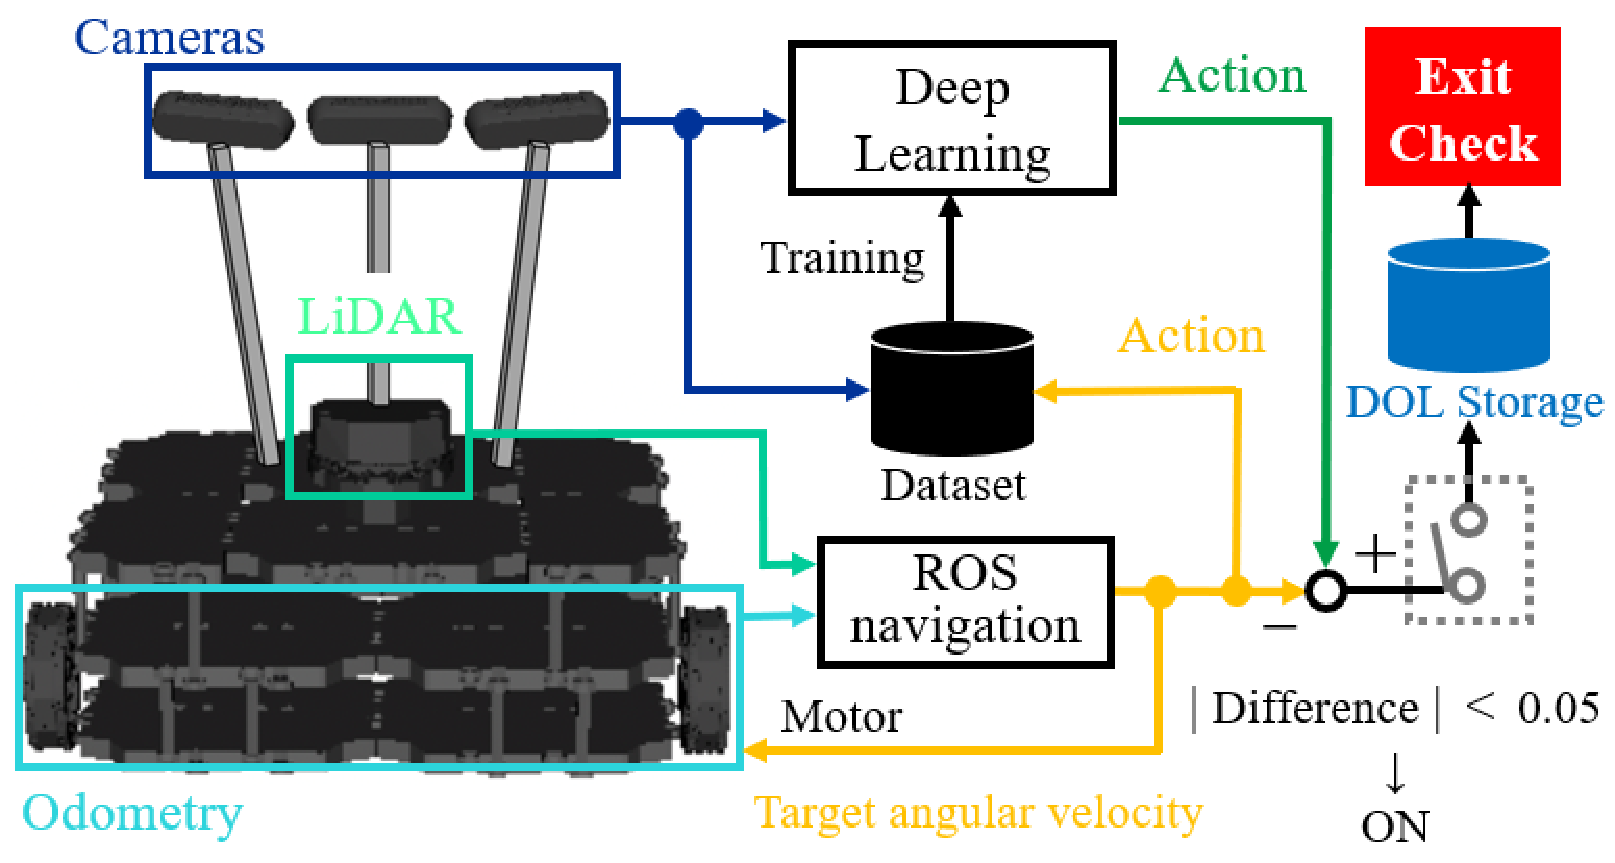
\includegraphics[height=47mm]{./pdf/moderu.pdf}
   \caption{Method to terminate training}
   \label{fig:5}
\end{figure}



\section{データセットの偏りの確認}
従来手法では,すべての経由点間でDOLの割合が 33%以上であれば,99%経路追従に成功する
様子が見られた\cite{imai2}.
ただし,目標経路に対して,常に同じ密度でデータセットを収集しているため,
目標経路の多くを占める直線的な経路では,過剰にデータを収集しているおそれがある.
経路の一部でも極端にデータの割合が多いと,割合の少ないデータはあまり学習されないため,
訓練打ち切りの指標を満たすのに多くの時間を要する.
そこで,前章で述べた学習を行い,それによって得た結果の一例から,収集および学習されるデータセットに
偏りがあるかを確認する.

\subsection{実験装置}
実験はシミュレータで行う.シミュレータには Gazebo\cite{gazebo},環境には Willow Garage を用いた.
ロボットには TurtleBot3\cite{TurtleBot3}にカメラを 3つ取り付けたモデルを用いた.

\subsection{実験方法}
実験では,はじめに地図に基づく経路追従を模倣学習する.
このとき,ロボットは\figref{fig:6}に示すような緑色の経由点を順次移動するが,
経由点の配置は先行研究\cite{imai2}と同じである.
ここで,各地点でデータがどの程度収集されたかを確認するため,
各経由点間に位置情報を加えたデータセットを収集する.
図の赤で示した部分は,先行研究において経路追従に多く失敗した地点である.
ただし,ロボットは位置情報は学習せず,従来と同様に画像から角速度のみを予測する.
学習後は,ロボットが収集および学習したデータセットの割合を可視化することで,
偏りがあるかを確認する.

\begin{figure}[h!]
  \centering
   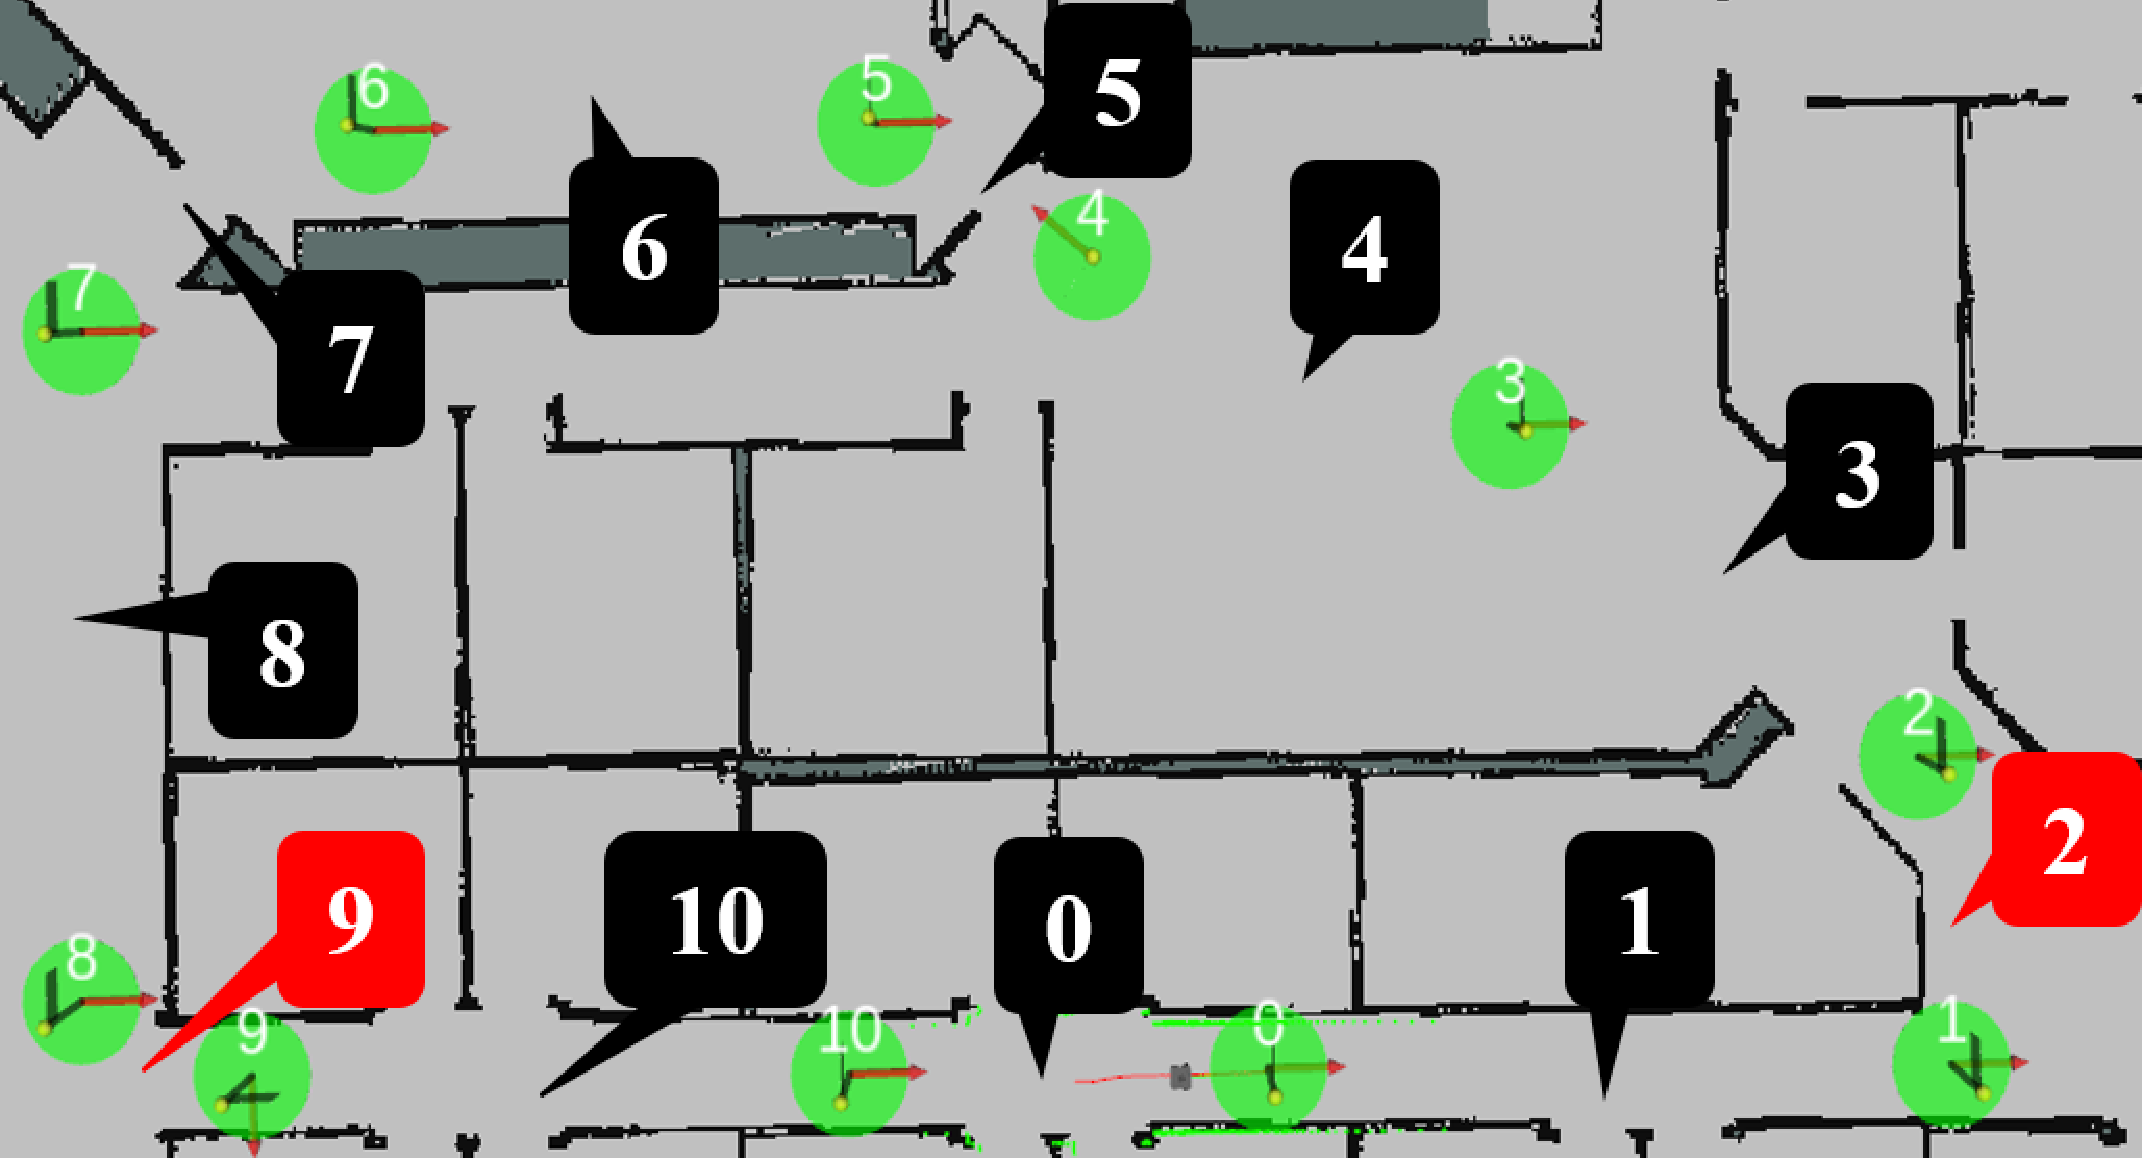
\includegraphics[height=40.5mm]{./pdf/location.pdf}
   \caption{Waypoints used in the experiment}
   \label{fig:6}
\end{figure}

\subsection{実験結果}
\figref{fig:8}に収集したデータセットの割合,\figref{fig:9}に学習に用いられたデータセットの割合を示す.
\figref{fig:8}より,先行研究で経路追従に失敗した地点である 9 番のデータセットが
他の地点と比べて少ないことがわかる.
また,\figref{fig:9}より,0 番や 1 番などの直線的な経路のデータが多く学習され,
9 番のデータセットがあまり学習されていないことがわかる.
つまり,目標経路の多くを占める直線的な経路では過剰にデータを収集しており,その結果,割合の
少ないデータがあまり学習されていない.そのため,経路全体で望む出力を得るための学習時間は長くなり,
効率的でないといえる.
以上から,収集および学習されるデータセットには偏りがあることが一例ではあるが確認された.

\begin{figure}[h!]
  \centering
   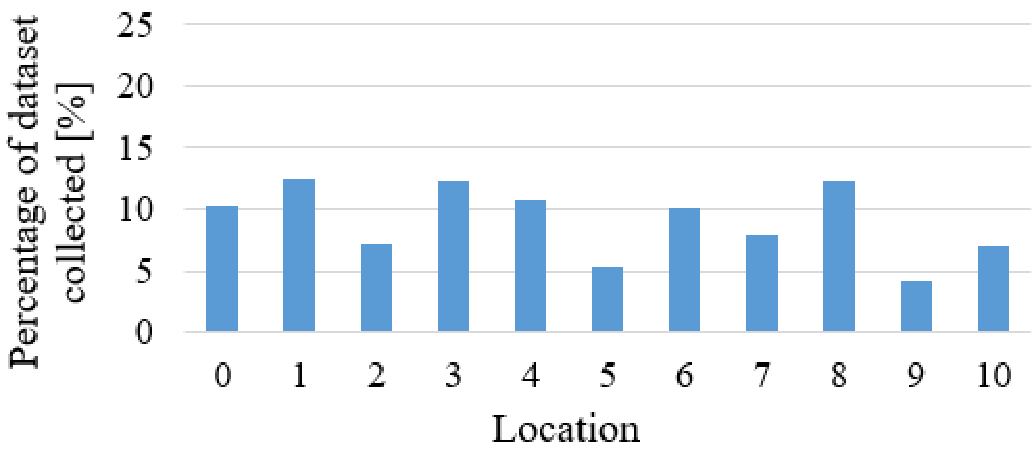
\includegraphics[height=33mm]{./pdf/set2.pdf}
   \caption{Precentage of dataset collected}
   \label{fig:8}
\end{figure}



\begin{figure}[h!]
  \centering
   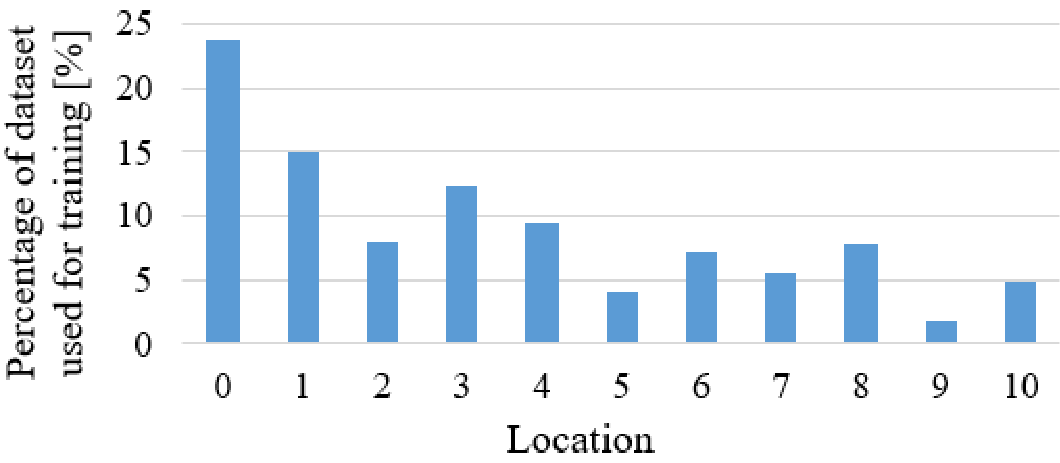
\includegraphics[height=33mm]{./pdf/gaku2.pdf}
   \caption{Precentage of dataset used for training}
   \label{fig:9}
\end{figure}


\section{提案手法}
4章の結果から,収集および学習されるデータセットには偏りがあることがわかった.
よって,データセットの収集密度を調整する手法を提案する.
\figref{fig:10}に提案手法を示す.従来手法では,学習時のロボットの並進速度は常に一定(0.2 m/s)
であったが,教師データとなる ROS navigation パッケージの目標角速度の値に応じて
ロボットの並進速度を可変にする仕組みを追加している.具体的には,目標角速度の絶対値が 0.1 rad/s 未満
であれば,ロボットの並進速度を従来の2倍(0.4 m/s)とし,0.1 rad/s 以上であれば,従来と同じ(0.2 m/s)
とする.なお,0.1 rad/s という値は,3つのカメラを用いるしきい値に由来する.
これにより,目標経路の多くを占める直線的な経路で過剰にデータを収集することを防ぐ効果が期待される.
それに伴い,学習されるデータセットの偏りも改善されることで,訓練打ち切りの指標を比較的早い段階で満たす
ことが期待される.


\begin{figure}[htbp]
  \begin{minipage}[t]{0.5\linewidth}
    \centering
    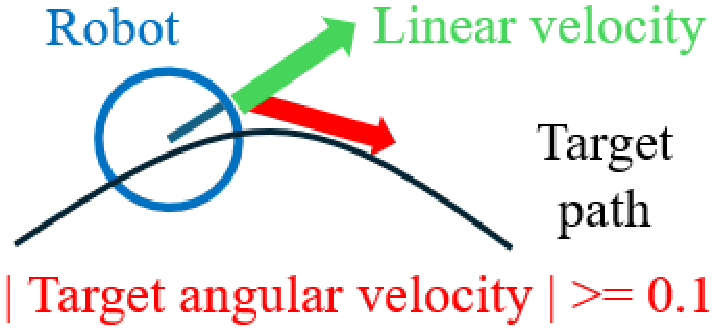
\includegraphics[keepaspectratio, scale=0.34]{./pdf/a2.pdf}
    \subcaption{Low speed}
  \end{minipage}
  \begin{minipage}[t]{0.5\linewidth}
    \centering
    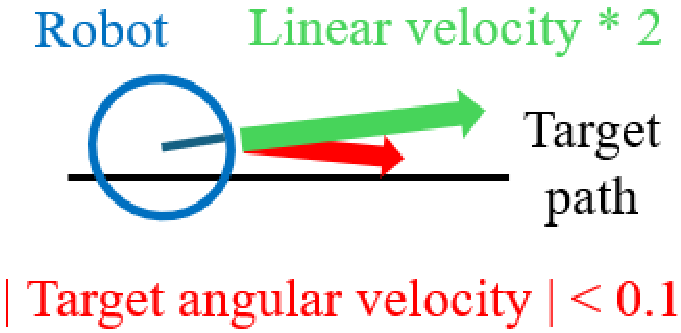
\includegraphics[keepaspectratio, scale=0.34]{./pdf/b.pdf}
    \subcaption{High speed}
  \end{minipage}
  \caption{Proposed method}
  \label{fig:10}
\end{figure}


\section{提案手法を用いた実験}

\subsection{実験装置,実験方法}
提案手法の有効性を検証するため,実験を行う.
実験装置や実験方法は 4章と同様である.
ただし,4章の実験とは異なり,学習後は訓練済みモデルを用いて経路追従できるかを確認する.
壁に衝突することなく,学習した経路を 1周することができれば成功とみなし,100 回実験する.
経路追従の成功率と訓練打ち切りステップ数,収集および学習したデータセットの割合から
提案手法の有効性を評価する.

\subsection{実験結果}
\subsubsection{経路追従の成功率}
\tabref{table:2}に経路追従の結果を示す.
結果的に,提案手法を用いても,従来手法と経路追従の成功率は変わらなかった.
ちなみに失敗した地点は,4.2節の\figref{fig:6}の 9番であり,従来手法において失敗した地点と同じであった.

\begin{table}[h!]
  \centering
  \caption{Number of successes in experiments}
  \label{table:2}
    \scalebox{0.96}[0.96] {
    \begin{tabular}{|l||c|}
      \hline
      Experiments & Number of successes \\
      \hline\hline
      Conventional method & 99/100 \\
      \hline
      Proposed method & 99/100\\
      \hline 
    \end{tabular} }
\end{table}

\subsubsection{訓練打ち切りステップ数}
\figref{fig:11}に手法ごとの 100回の訓練打ち切りステップ数の分布を示す.
従来手法では,最短で 4000 から 6000 ステップの訓練を必要としたのに対し,提案手法では,
最短で 2000 から 4000 ステップで訓練を終了しているものがある.
つまり,提案手法を用いた方が訓練打ち切りの指標を早くに満たすことができるといえる.
ちなみに,従来手法の平均ステップ数は約 6262ステップ,提案手法の平均ステップ数は
約 4742ステップであり,平均で約 1500ステップ(約5分)の訓練時間を短縮できた.
6.2.1 項の結果より,双方で経路追従の成功率は変わらないため,提案手法は経路追従の成功率を損なわずに
訓練時間を短縮できるといえる.

\begin{figure}[htbp]
  \begin{minipage}[t]{0.5\linewidth}
    \centering
    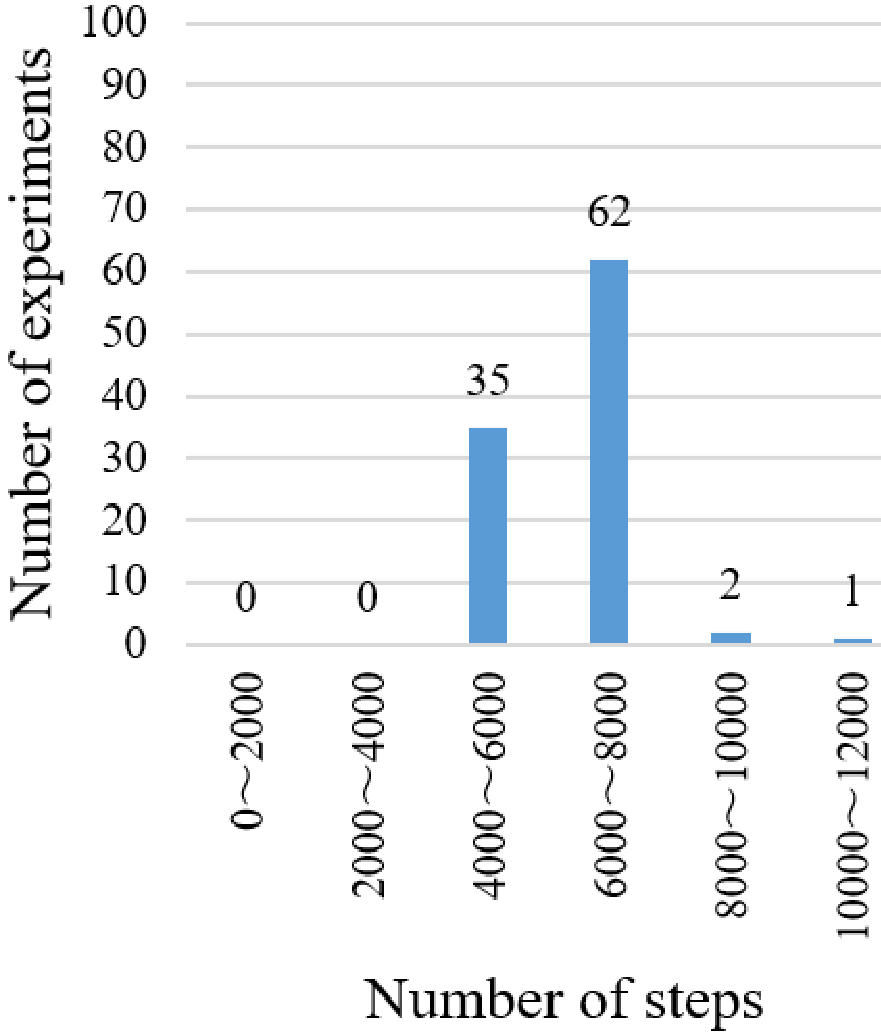
\includegraphics[keepaspectratio, scale=0.27]{./pdf/c.pdf}
    \subcaption*{\hspace*{2.5zw}(a) Conventional method}
  \end{minipage}
  \begin{minipage}[t]{0.5\linewidth}
    \centering
    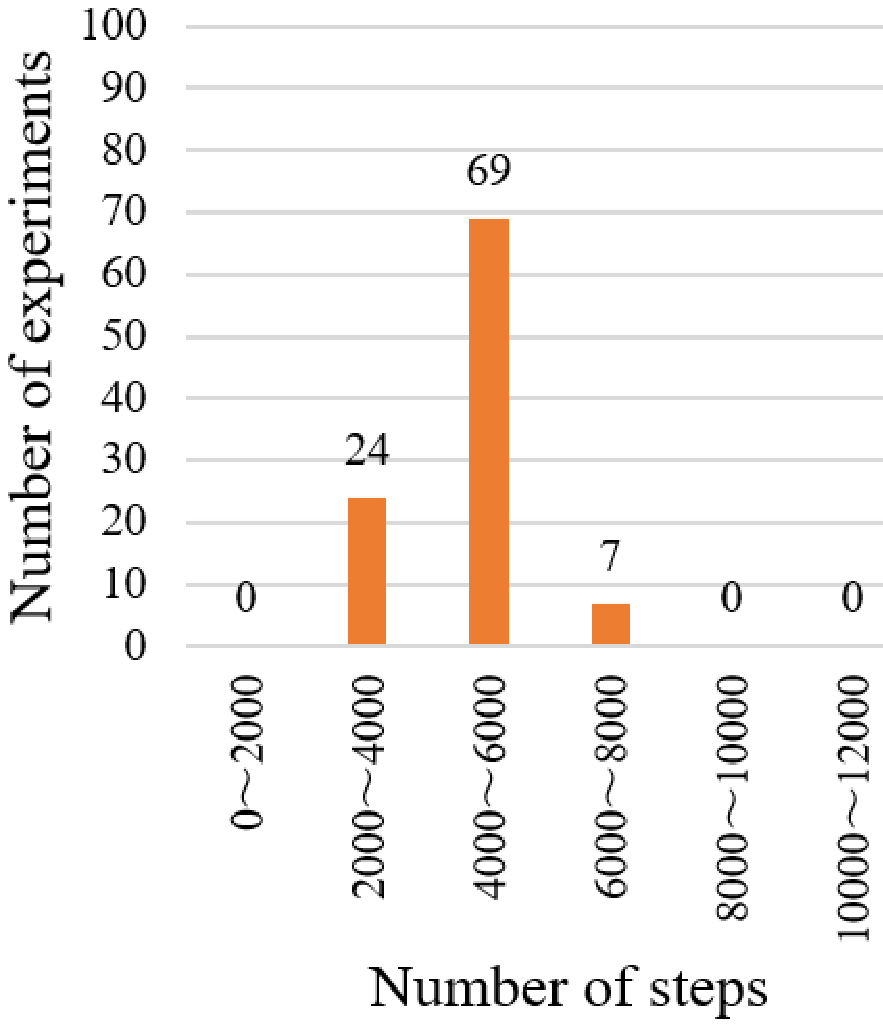
\includegraphics[keepaspectratio, scale=0.273]{./pdf/p.pdf}
    \subcaption*{\hspace*{2.5zw}(b) Proposed method}
  \end{minipage}
  \caption{Distribution of the number of steps terminated}
   \label{fig:11}
\end{figure}


\subsubsection{収集および学習したデータセットの割合}
\figref{fig:12}に収集したデータセットの割合,\figref{fig:13}に学習に用いられたデータセットの割合を示す.
これらは,従来手法と提案手法で成功した 10 回ずつの結果を平均したものである.
\figref{fig:12},\figref{fig:13}ともに,提案手法では 0 番や 1番など,目標経路の多くを占める直線的な経路
のデータの割合が少なくなり,2 番や 9 番など,曲がり角周辺のデータの割合が多くなったことがわかる.
つまり,データセットの収集密度が改善されたことで,学習に用いられるデータセットの偏りも改善することが
できたといえる.また,それにより学習を効率化することができたといえる.

\begin{figure}[h!]
  \centering
   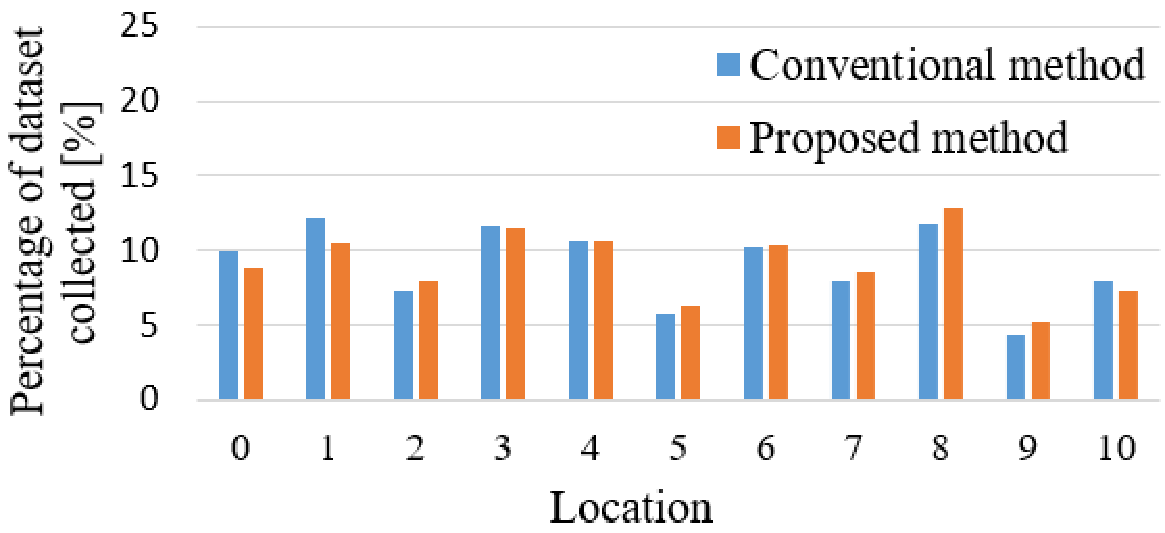
\includegraphics[height=35mm]{./pdf/dataset_pro2.pdf}
   \caption{Precentage of dataset collected}
   \label{fig:12}
\end{figure}

\begin{figure}[h!]
  \centering
   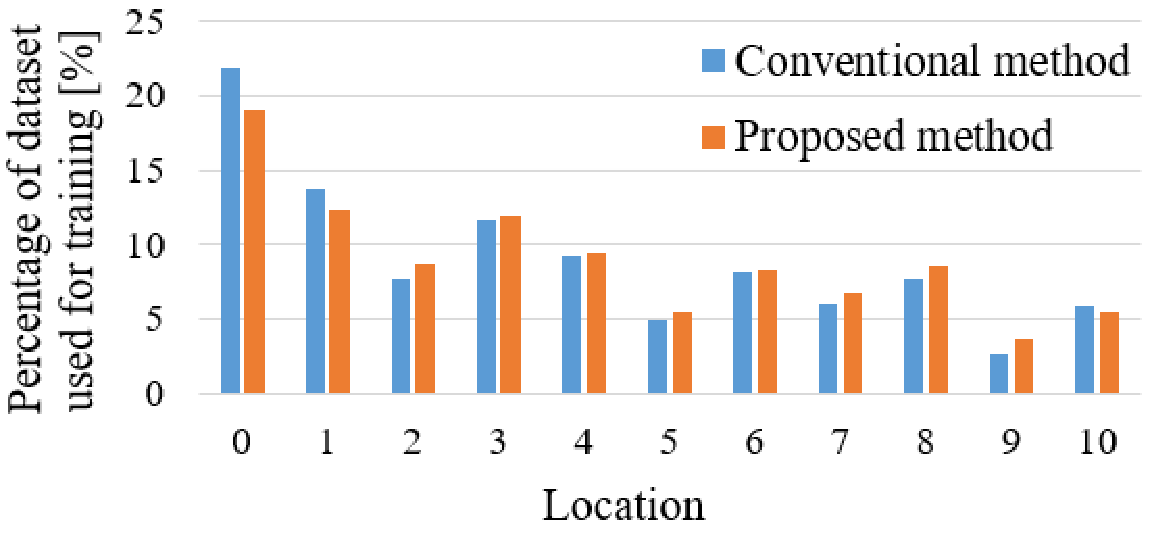
\includegraphics[height=35mm]{./pdf/gaku_pro2.pdf}
   \caption{Precentage of dataset used for training}
   \label{fig:13}
\end{figure}



\section{結言}
本稿では,従来から提案する経路追従行動の模倣手法における実験結果の一例を取り上げ,
収集および学習されるデータセットには偏りがあることを一例ではあるが確認した.
そのうえで,データセットの収集密度を調整し,学習を効率化するために,ロボットの並進速度を教師データの
値に応じて可変にする手法を提案した.その後,シミュレータでの実験により提案手法の有効性を検証した.
結果的に,提案手法は従来手法に比べて,データの収集密度を改善し,学習に用いられるデータの偏りを改善できた.
それにより,訓練打ち切りの指標を早くに満たすことができる傾向が見られたため,
学習を効率化するうえで有効であることが確認された.\\

\vspace*{0.3zh}

\footnotesize
\begin{thebibliography}{99}

\bibitem{okada}
岡田眞也, 清岡優祐, 上田隆一, 林原靖男, “視覚と行動の end-to-end 学習により経路追従行動をオンラインで模倣する手法の提案”, 計測自動制御学会 \textit{SI} 部門講演会 \textit{SICE-SI2020} 予稿集, pp.1148-1152, 2020.

\bibitem{okada2}
岡田眞也, 清岡優祐, 春山健太, 上田隆一, 林原靖男, “視覚と行動の end-to-end 学習により経路追従行動をオンラインで模倣する手法の提案 -経路追従行動の修正のためにデータセットを動的に追加する手法の検討-”, 計測自動制御学会 \textit{SI} 部門講演会 \textit{SICE-SI2021} 予稿集, pp.1066-1080, 2021.

\bibitem{kiyooka}
清岡優祐, 岡田眞也, 岩井一輝, 上田隆一, 林原靖男, “視覚と行動の end-to-end 学習により経路追従行動をオンラインで模倣する手法の提案 -データセットと生成された経路追従行動の解析-”, 計測自動制御学会 \textit{SI} 部門講演会 \textit{SICE-SI2021} 予稿集, pp.1071-1075, 2021.

\bibitem{off_load}
U. Muller, J. Ben, E. Cosatto, B. Flepp, and Y. Cun, “Off-Road Obstacle Avoidance through End-to-End Learning”, \textit{Advances in neural information processing systems}, Vol. 18, 2005.

\bibitem{Moridian}
Moridian, Barzin, Anurag Kamal, and Nina Mahmoudian, “Learning Navigation Tasks from Demonstration for Semi-autonomous Remote Operation of Mobile Robots”, \textit{2018 IEEE International Symposium on Safety, Security, and Rescue Robotics (SSRR)}, pp.1-8, 2018.

\bibitem{Bojarski}
Bojarski, Mariusz, \textit{et al}., “End to end learning for self-driving cars”, \textit{arXiv:1604.08316}, 2016.

\bibitem{imai}
今井悠月, 清岡優祐, 春山健太, 上田隆一, 林原靖男, “視覚と行動の end-to-end 学習により経路追従行動をオンラインで模倣する手法の提案 -経路への復帰行動の解析と復帰行動を強化する教師データ収集法の検討-”, 日本機械学会ロボティクス・メカトロニクス講演会'23 予稿集, 2P2-G05(2023).

\bibitem{fuji}
藤原柾, 春山健太, 馬場琉生, 上田隆一, 林原靖男, “視覚と行動のend-to-end 学習により経路追従行動をオンラインで模倣する手法の提案 -実環境における経路選択機能の検証と学習時間の短縮化の検討-”, 日本機械学会ロボティクス・メカトロニクス講演会'23予稿集, 2P2-G06(2023)

\bibitem{takahashi}
\CID{8705}橋祐樹, 白須和暉, 藤原柾, 上田隆一, 林原靖男, “視覚と行動のend-to-end 学習による経路追従行動の模倣”, 日本機械学会ロボティクス・メカトロニクス講演会'23予稿集, 2P1-G07(2023)

\bibitem{imai2}
今井悠月, 落合拓海, 白須和暉, 上田隆一, 林原靖男, “視覚と行動のend-to-end 学習により経路追従行動をオンラインで模倣する手法の提案 -モデルの評価に基づく訓練ステップ数の決定-”, 1B1-04, \textit{SI2023}, (2023)

\bibitem{navigation}
ros-planning, navigation リポジトリ\\
https://github.com/ros-planning/navigation.\\
(最終閲覧日 : \today)

\bibitem{gazebo}
Nathan Koenig and Andrew Howard, “Design and use paradigms for gazebo, an open-source multi-robot simulator”, \textit{2004 IEEE/RSJ International Conference on Intelligent Robots and Systems (IROS)}, Vol.3, pp.2149-2154, 2004.

\bibitem{TurtleBot3}
Erico Guizzo and Ackerman Evan, “The TurtleBot3 Teacher [Resources Hands On]”, \textit{IEEE Spectrum}, Vol.54, pp.19-20, August 2017.

\end{thebibliography}


\normalsize
\end{document}
